\section{Don’t Augment Me\protect\footnotemark[1]}\label{results:dont-augment-me}

\footnotetext[1]{Results from this section are also part of the paper submitted to the \textit{"Thirty-fifth Conference on Neural Information Processing Systems", NeurIPS 2021} called \textit{"Don’t Augment Me: On the Robustness of Saliency Methods"}. At the moment of writing this thesis, the paper is under the review process. The paper was written in collaboration with Piotr Mazurek.}

\vspace{-1.5\baselineskip}
\begin{figure}[ht]
  \centering
  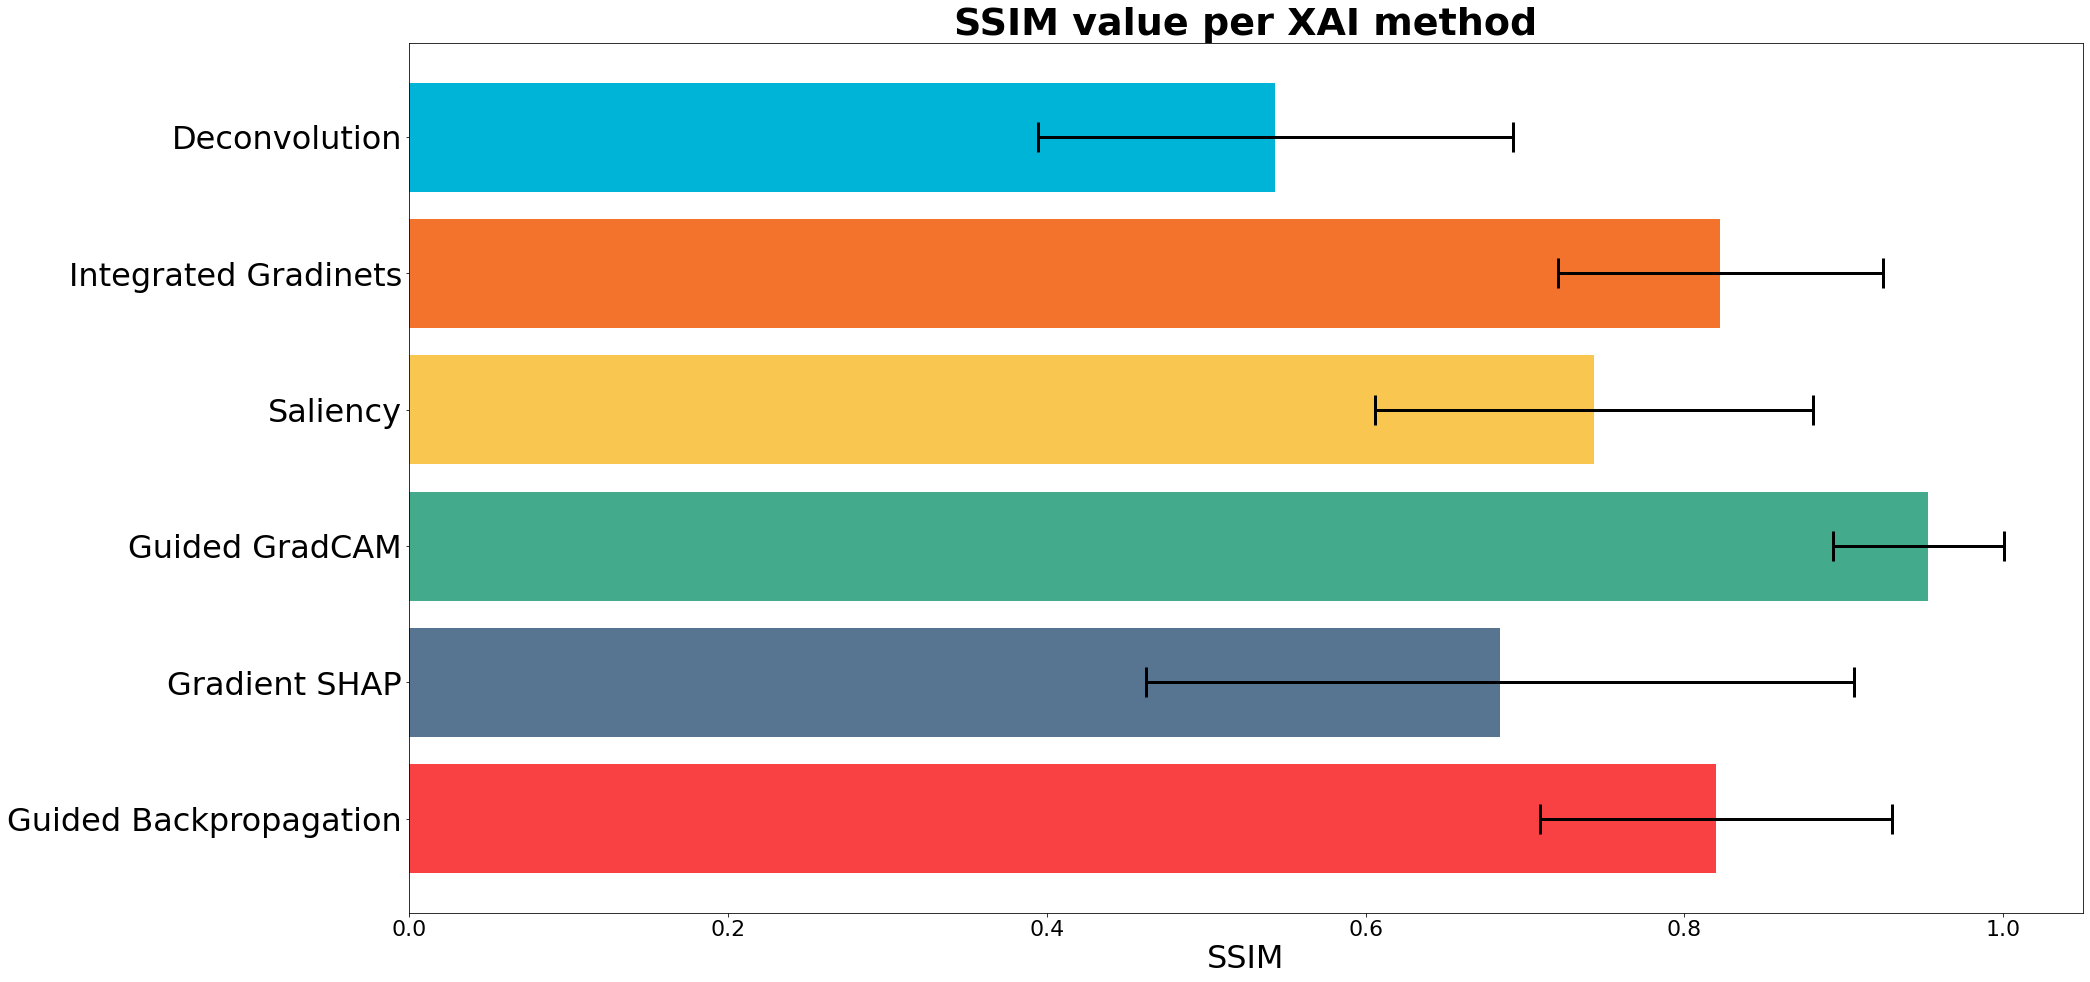
\includegraphics[width=0.8\textwidth]{results/augment-img/results-all.png}
  \caption{Average SSIM values per attribution method. Each bar represents a methods' mean value of SSIM. These mean values exclude examples when the classification score of the augmented image is outside the $threshold$ of a non-augmented image. Because the score is independent of the attribution method, all mean values are calculated from exactly the same images and augmentations.}\label{fig:SSIM-mean-std}
\end{figure}

\vspace{-1.5\baselineskip}
\begin{wrapfigure}{R}{0.62\textwidth}
%   \setlength{\belowcaptionskip}{-6pt}
 \centering
 \begin{subfigure}{.18\textwidth}
    \centering
    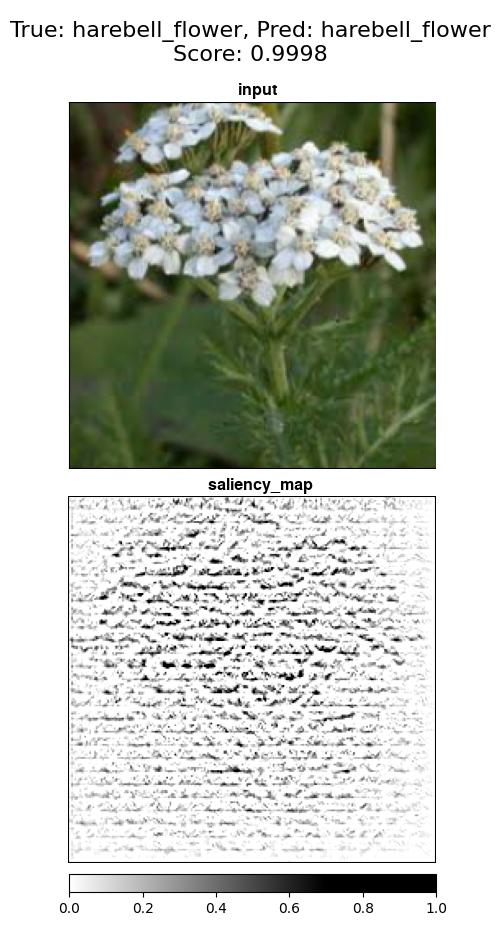
\includegraphics[width=\textwidth]{results/augment-img/20-0-64-rotation-0-harebell_flower-harebell_flower_vert.jpg}
    \caption{Original image}\label{fig:original-harebell}
\end{subfigure}
 \begin{subfigure}{.18\textwidth}
    \centering
    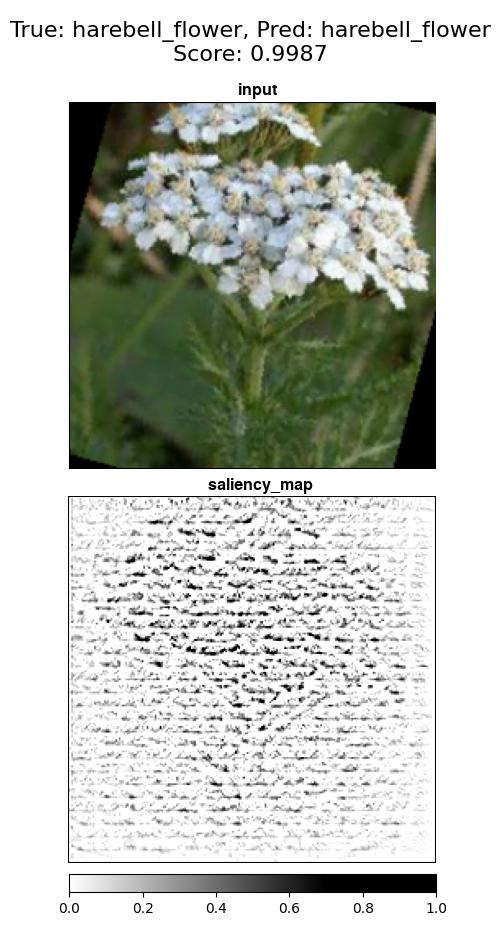
\includegraphics[width=\textwidth]{results/augment-img/20-2-64-rotation--15-harebell_flower-harebell_flower_vert.jpg}
    \caption{Rotation of -15°}\label{fig:rotated-harebell}
\end{subfigure}
 \begin{subfigure}{.22\textwidth}
    \centering
    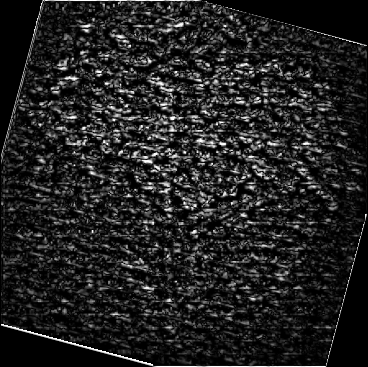
\includegraphics[width=\textwidth]{results/augment-img/harebell_flower-differences.png}
    \caption{Attribution difference}\label{fig:harebell-differences}
\end{subfigure}

 \caption{Visualisation of attributions for \textit{Harebell Flower} image from Plants \cite{plants-dataset} tested on ResNet18 \cite{he2015deep} trained on 100\% of the training dataset. SSIM value for this pair: \textbf{0.2518}. The difference between attribution of rotated image (Fig. \ref{fig:rotated-harebell}) and the rotated attribution of the original image (Fig. \ref{fig:original-harebell}). Black color indicates the same values, and the white color indicates differences.}\label{fig:xai-harebell-deconv}
\end{wrapfigure}

\hfill \break

After calculating mean SSIM scores per tested method, we can clearly see large discrepancies between XAI methods. The method with the highest average score (Fig. \ref{fig:SSIM-mean-std}) is \textit{Guided GradCAM}, which achieved an average of $0.95$ ($\sigma = 0.05$). On the other hand, we have \textit{Deconvolution} with an average score of only $0.54$ ($\sigma = 0.15$). In terms of SSIM value, this difference is larger than expected, and additional explanation is needed.

\vspace{\baselineskip}

When creating an attribution, the Deconvolution method is using a reverse convolutional operation (building a reverse network, described in Section \ref{section:deconvolution}). Because the output from that network ends with a filter, it creates attributions from basic geometric shapes (see Fig. \ref{fig:xai-harebell-deconv}). This approach has a huge disadvantage when trying to compare attributions of rotated images (unless rotation is defined within a convolutional filter). From a wider perspective, when we look at Figures \ref{fig:original-harebell} and \ref{fig:rotated-harebell}, they look very similar. When we look closer and try to actually compare attribution from Figure \ref{fig:rotated-harebell} with rotated attribution from Figure \ref{fig:original-harebell}, we can see that lines are not aligned with each other (see Figure \ref{fig:harebell-differences}).

\vspace{\baselineskip}

This issue is better visualized when compare the mean value of Deconvolition from Figure \ref{fig:SSIM-mean-rotation} with the value from Figure \ref{fig:SSIM-mean-filters}. There is a clear difference between means (and also standard deviations), with the second Figure having the Deconvolution mean closer to the rest of the methods.

\begin{figure}[ht]
  \centering
  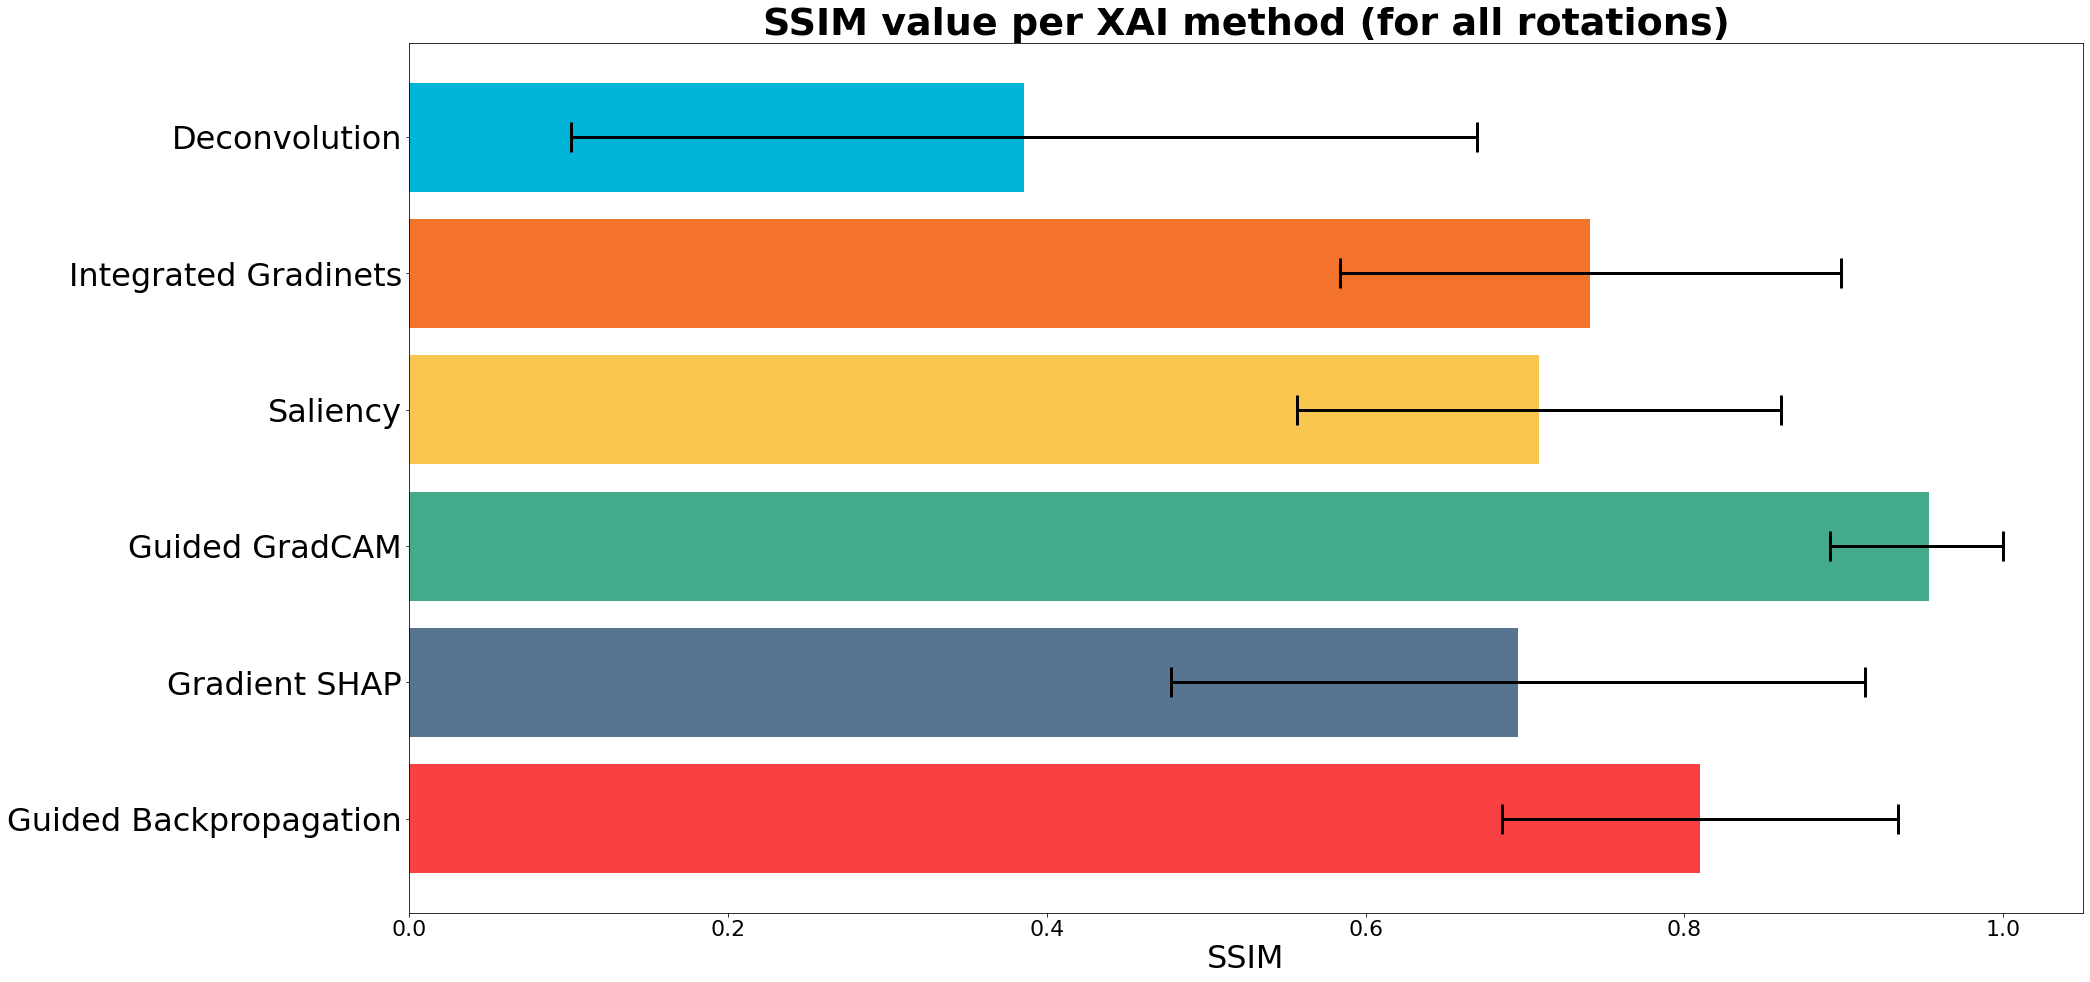
\includegraphics[width=0.8\textwidth]{results/augment-img/rotation-all.png}
  \caption{Average SSIM values per attribution method. Each bar represents a methods' mean value of SSIM. Values used to calculate the mean value are restricted to come only from images augmented by applying rotations. The detailed version of this chart is available in Figure \ref{fig:SSIM-all-rotation}.}\label{fig:SSIM-mean-rotation}
\end{figure}


\begin{figure}[ht]
  \centering
  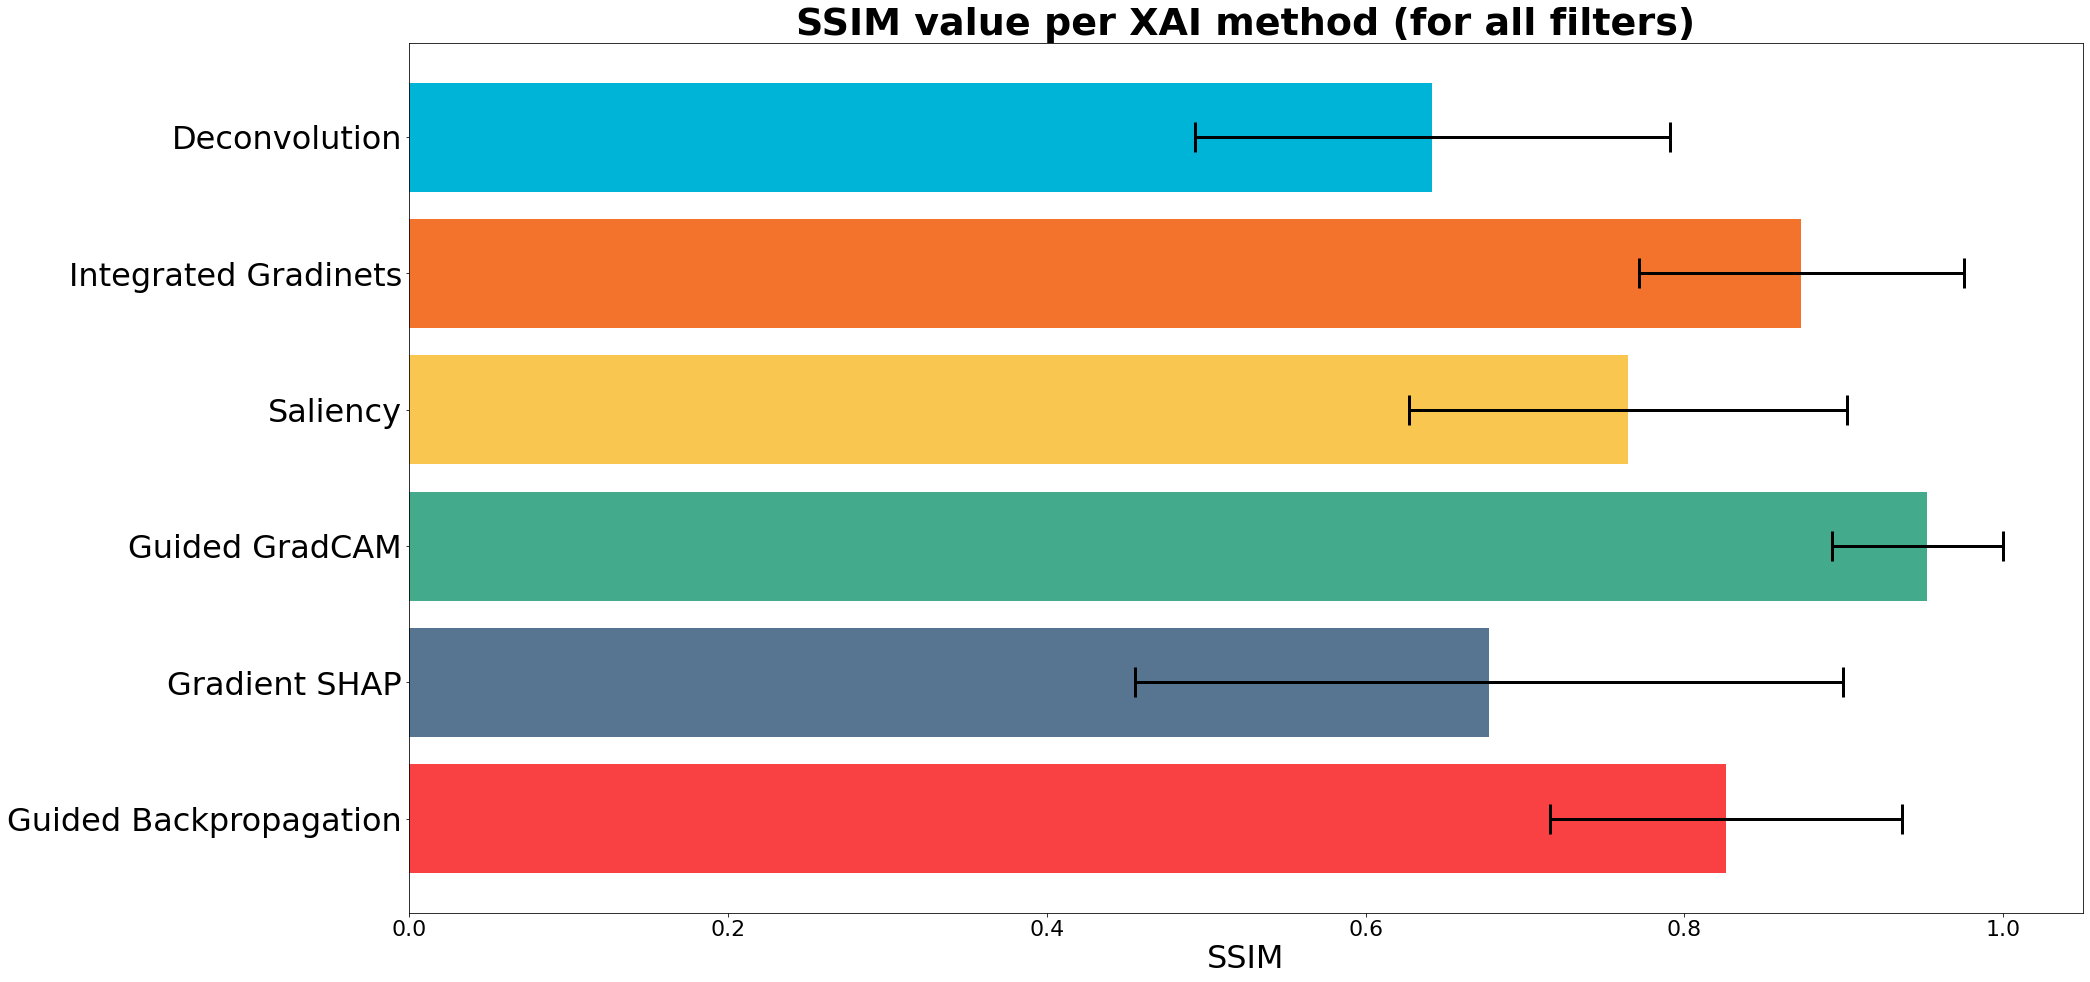
\includegraphics[width=0.8\textwidth]{results/augment-img/filters-all.png}
  \caption{Average SSIM values per attribution method. Each bar represents a methods' mean value of SSIM. Values used to calculate the mean value are restricted to come only from images augmented by applying filters. The detailed version of this chart is available in Figure \ref{fig:SSIM-all-filters}.}\label{fig:SSIM-mean-filters}
\end{figure}

The values of Guided GradCAM are closest to $1.0$ (see Fig. \ref{fig:SSIM-mean-std}), which would indicate the ideal method (no changes in attributions). A mean score of $0.95$ might be confusing and provide a false sense of trust in the method. A good example can be seen in Figure \ref{fig:xai-tiramisu}. Two attributions have the SSIM score of $0.9357$, but the visual comparison of those two images allows us to see major differences. The main difference is the number of details shown in Figure \ref{fig:norm-tiramisu}. Both images achieve almost the same score, so the augmentation does not cause the model to change its decision. An average score for the Guided GradCAM method is just $0.0143$ away from the score achieved by this example.

\begin{wrapfigure}{R}{0.42\textwidth}
%   \setlength{\belowcaptionskip}{-2pt}
 \centering
 \begin{subfigure}{.2\textwidth}
    \centering
    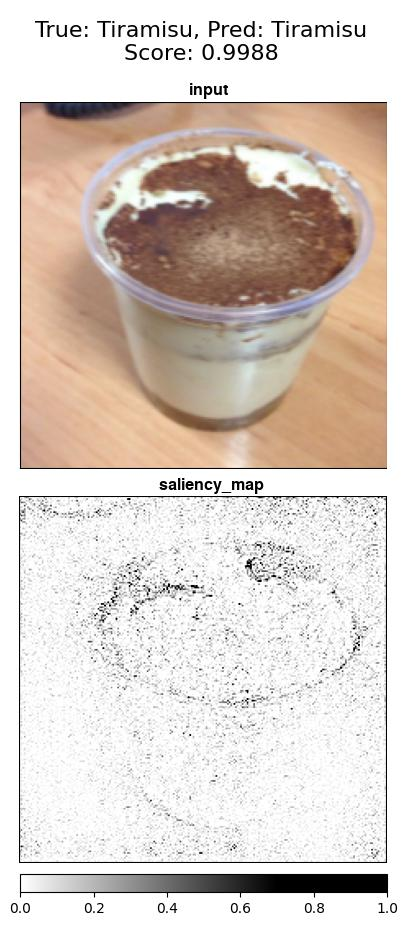
\includegraphics[width=\textwidth]{results/augment-img/19-0-98-none-Tiramisu-Tiramisu_vert.jpg}
    \caption{Original image}\label{fig:original-tiramisu}
\end{subfigure}
 \begin{subfigure}{.2\textwidth}
    \centering
    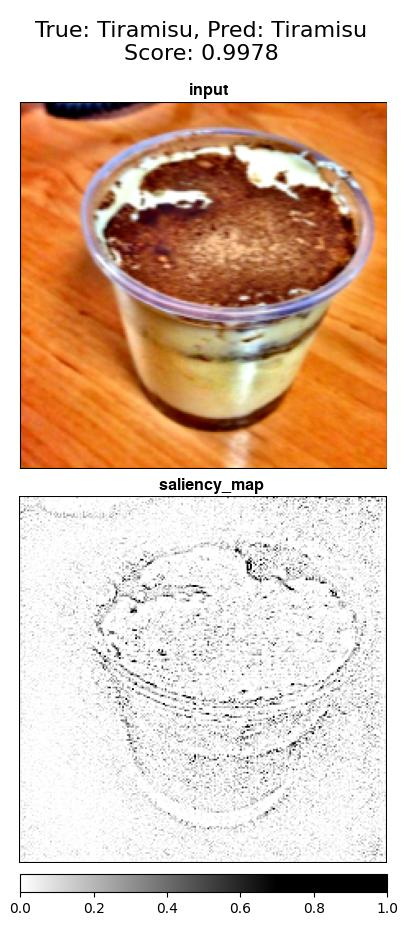
\includegraphics[width=\textwidth]{results/augment-img/19-2-98-normalize_local 8,10-Tiramisu-Tiramisu_vert.jpg}
    \caption{Local Norm}\label{fig:norm-tiramisu}
\end{subfigure}

 \caption{Visualisation of attributions done by GradCAM \cite{selvaraju2017grad} for \textit{Tiramisu} image from Food101 \cite{food101} tested on DenseNet121 \cite{huang2017densely} trained on 100\% of the training dataset. SSIM value for this pair: \textbf{0.9357}.}\label{fig:xai-tiramisu}
 \vspace{-38pt}
\end{wrapfigure}

\vspace{\baselineskip}

To provide an overview of the used method, we can look at Figure \ref{fig:attrib-samples}. This overview does not contain all types of examples, which are stored separately and linked in Appendix \ref{appendix:attribution-samples}. Each pair of rows represents a set of augmentations (without rotations) per image per the XAI method. Augmentations names are visible above the examples, and all the predictions of the augmented images are within the $threshold$ of the \textit{"none"} image (first column). This is a slightly more restrictive list than the one used in calculating SSIM values. It is easier to pick examples by searching for the pair of images within the $threshold$ than to find a set of 5 examples where all of them are within the $threshold$. That is why in this list, there are fewer visually different attributions.

\vspace{\baselineskip}

Every set of augmentations contain at least one example where the attribution is significantly different than the original one. Lets start with the Deconvolution (\textit{Rottweiler}). Two augmentations (\textit{Freaky Details} and \textit{Local Norm}) are causing the attribution method to display more details than the original one. Some of those details are related to the dog, but the rest is focusing on the window shutter. A similar problem with focusing on the different parts of the image can be seen in the \textit{Dandellion} example generated with Integrated Gradients \cite{sundararajan2017axiomatic}. Only \textit{Mighty Details} attribution stays the same (visually) when attributions for the rest of augmentations are changing their focus of the plant.

\vspace{\baselineskip}

The main problem with these changes in the attribution is that they are nondeterministic. One augmentation might cause a method to focus on the details more, and the same augmentation might create the opposite behavior when applied on a different image (or even the same image but a different model). Some of the changes are minor and can be ignored (like the two just described), but there are more visually outstanding examples.

\vspace{\baselineskip}

Let us look on the examples from Guided GradCAM \cite{selvaraju2017grad}, GradSHAP \cite{erion2019learning}, and Saliency \cite{simonyan2014deep}. An example attributed by Guided GradCAM changes its attribution significantly when the \textit{Mighty Details} filter is applied. This change is significant enough to change our understanding of what is important for a model in predicting the \textit{sussex\_spaniel} class. The attribution of the original image focuses mostly on the dog's head when the attribution of the augmented image focuses on the whole body. The same applies to the example attributed by GradSHAP. Here, the attribution of the original image points to the dog's nose when four other attributions of the augmented images are pointing to other parts of the animal (like ears and eyes). The example from the Saliency method shows different behavior. This time, when applying the \textit{Local Norm} filter on the image, the attribution ignores some of the details in comparison with the original attribution.

\vspace{\baselineskip}

The most relevant example is that generated with the help of GBP \cite{springenberg2014striving}. In that example, the model predicts the \textit{black\_widow} class for all images. The attribution of most is focused on the scene details and the character of Black Widow. This changes when \textit{Local Norm} is applied, and the attribution starts to display a lot of details of the Hulk character. A shift like that might be dangerous when the understanding of the models' decisions is critical.


\begin{figure}[ht]
  \centering
  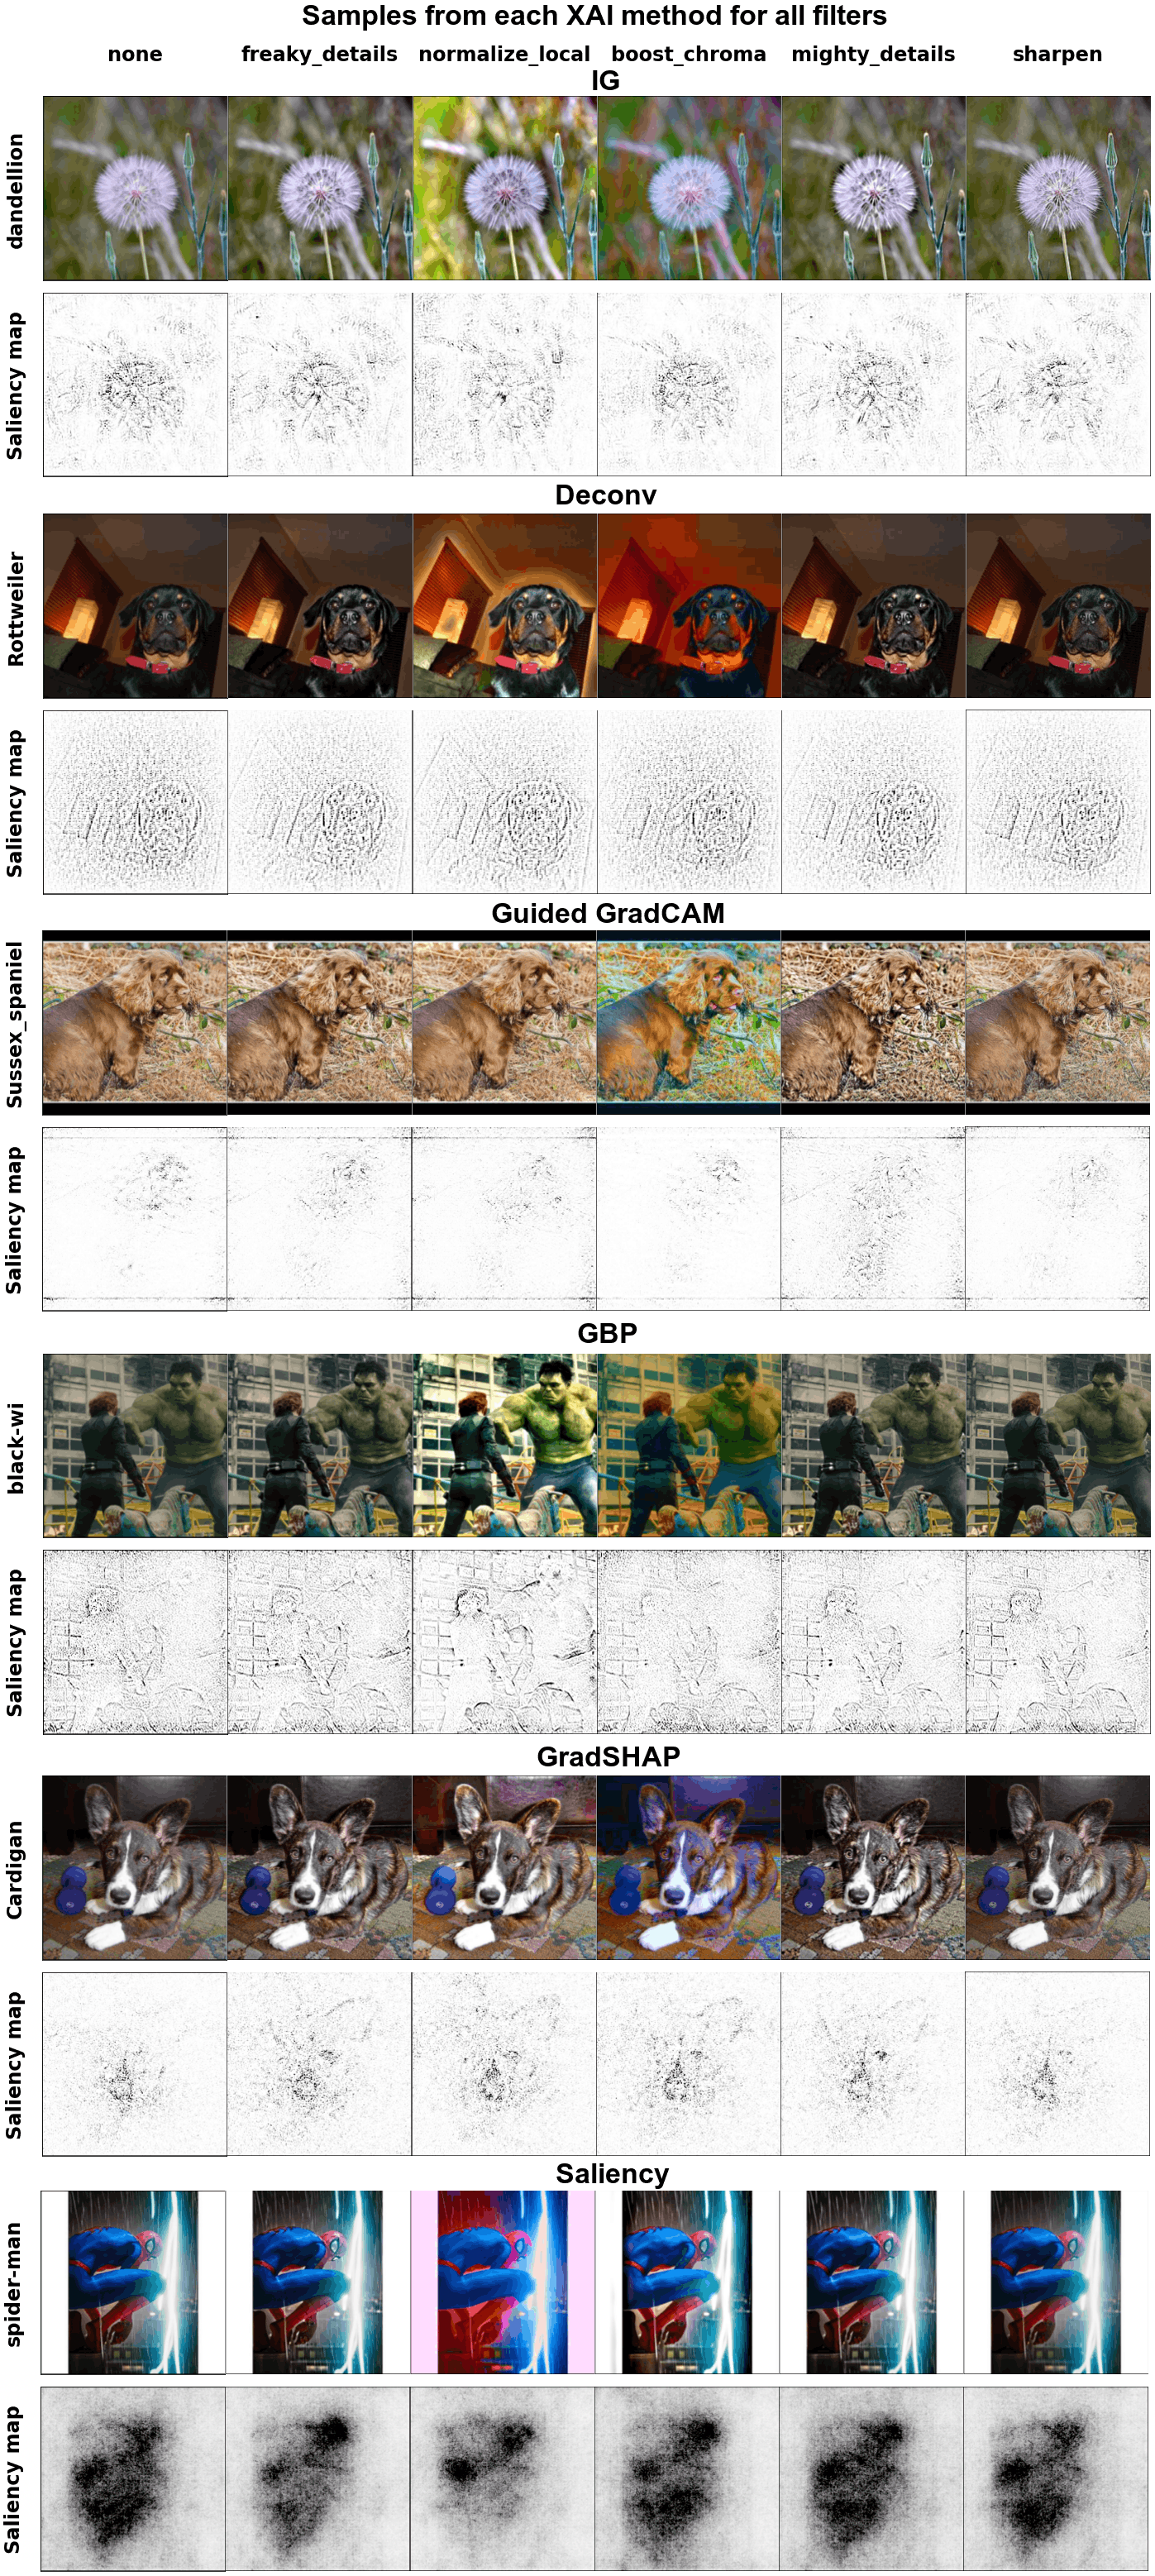
\includegraphics[width=0.58\textwidth]{results/augment-img/all_methods_samples.png}
  \caption{Augmentation attribution samples for every method. Samples are selected to all be within the $threshold$ of the original image. Each row represents samples for all augmentations except rotations. More samples available in Appendix \ref{appendix:attribution-samples}}\label{fig:attrib-samples}
\end{figure}
